%%%%% Description: 1+3-framework %%%%%
%%%%% Created: July 24, 2016 %%%%%
%%%%% Author: Hengfeng Wei (hengxin) %%%%%

\documentclass{standalone}

\usepackage{tikz}
\usetikzlibrary{positioning, shapes, shapes.geometric, backgrounds, fit, arrows.meta, calc}
\usepackage{varwidth}

\begin{document}
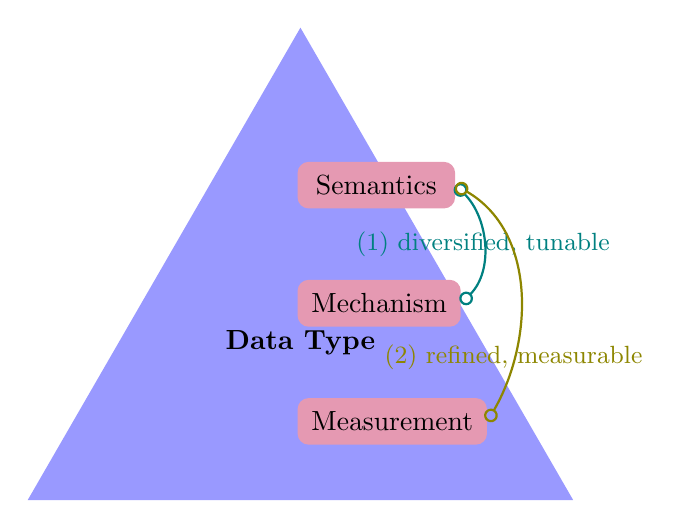
\begin{tikzpicture}[fnode/.style = {fill = purple!40, rectangle, rounded corners, inner sep = 5pt, minimum width = 2.0cm},
	conn/.style = {<->, >={Circle[open]}, thick, #1}]
  % 1: data type
  \node (dt) [regular polygon, regular polygon sides = 3, 
  	fill = blue!40, inner sep = 5pt, minimum size = 8.0cm] {\bf Data Type};
  
  % 3: semantics, mechanism, and measurement
  \node (mechanism) [fnode] at (1.0cm, 0.5cm) {Mechanism};
  \node (semantics) [fnode, above = 1.5cm of mechanism.west, anchor = west] {Semantics};
  \node (measurement) [fnode, below = 1.5cm of mechanism.west, anchor = west] {Measurement};

  % 1+3: semantics + mechanism; semantics + measurement
  \draw[conn = teal] (semantics.east) to [out = -45, in = 45] node[font = \small] {(1) diversified, tunable} (mechanism.east);
  \draw[conn = olive] (semantics.east) to [out = -30, in = 60] node[near end, font = \small] {(2) refined, measurable} (measurement.east);
\end{tikzpicture}
\end{document}
